\documentclass[11pt,fleqn, oneside,openany]{book} % Default font size and left-justified equations

% use this list: https://www.educative.io/blog/google-coding-interview

%%%%%%%%%%%%%%%%%%%%%%%%%%%%%%%%%%%%%%%%%%%%
%               Structure
%%%%%%%%%%%%%%%%%%%%%%%%%%%%%%%%%%%%%%%%%%%%
%%%%%%%%%%%%%%%%%%%%%%%%%%%%%%%%%%%%%%%%%
% The Legrand Orange Book
% Structural Definitions File
% Version 2.0 (9/2/15)
%
% Original author:
% Mathias Legrand (legrand.mathias@gmail.com) with modifications by:
% Vel (vel@latextemplates.com)
% 
% This file has been downloaded from:
% http://www.LaTeXTemplates.com
%
% License:
% CC BY-NC-SA 3.0 (http://creativecommons.org/licenses/by-nc-sa/3.0/)
%
%%%%%%%%%%%%%%%%%%%%%%%%%%%%%%%%%%%%%%%%%

%----------------------------------------------------------------------------------------
%	VARIOUS REQUIRED PACKAGES AND CONFIGURATIONS
%----------------------------------------------------------------------------------------

\usepackage[top=3cm,bottom=3cm,left=3cm,right=3cm,headsep=10pt,a4paper]{geometry} % Page margins

\usepackage{graphicx} % Required for including pictures
\graphicspath{{images/}} % Specifies the directory where pictures are stored

\usepackage{lipsum} % Inserts dummy text

\usepackage{tikz} % Required for drawing custom shapes

\usepackage[english]{babel} % English language/hyphenation

\usepackage{enumitem} % Customize lists
\setlist{nolistsep} % Reduce spacing between bullet points and numbered lists

\usepackage{booktabs} % Required for nicer horizontal rules in tables

\usepackage{xcolor} % Required for specifying colors by name
\definecolor{ocre}{RGB}{243,102,25} % Define the orange color used for highlighting throughout the book

%----------------------------------------------------------------------------------------
%	FONTS
%----------------------------------------------------------------------------------------

\usepackage{avant} % Use the Avantgarde font for headings
%\usepackage{times} % Use the Times font for headings
\usepackage{mathptmx} % Use the Adobe Times Roman as the default text font together with math symbols from the Sym­bol, Chancery and Com­puter Modern fonts

\usepackage{microtype} % Slightly tweak font spacing for aesthetics
\usepackage[utf8]{inputenc} % Required for including letters with accents
\usepackage[T1]{fontenc} % Use 8-bit encoding that has 256 glyphs

%----------------------------------------------------------------------------------------
%	BIBLIOGRAPHY AND INDEX
%----------------------------------------------------------------------------------------

\usepackage[citestyle=numeric,sorting=nyt,sortcites=true,autopunct=true,babel=hyphen,hyperref=true,abbreviate=false,backref=true,backend=biber]{biblatex}
\addbibresource{sources/bibliography.bib}
\defbibheading{bibempty}{}

\usepackage{calc} % For simpler calculation - used for spacing the index letter headings correctly
\usepackage{makeidx} % Required to make an index
\makeindex % Tells LaTeX to create the files required for indexing

%----------------------------------------------------------------------------------------
%	MAIN TABLE OF CONTENTS
%----------------------------------------------------------------------------------------

\usepackage{titletoc} % Required for manipulating the table of contents

\contentsmargin{0cm} % Removes the default margin

% Part text styling
\titlecontents{part}[0cm]
{\addvspace{20pt}\centering\large\bfseries}
{}
{}
{}

% Chapter text styling
\titlecontents{chapter}[1.25cm] % Indentation
{\addvspace{12pt}\large\sffamily\bfseries} % Spacing and font options for chapters
{\color{ocre!60}\contentslabel[\Large\thecontentslabel]{1.25cm}\color{ocre}} % Chapter number
{\color{ocre}}  
{\color{ocre!60}\normalsize\;\titlerule*[.5pc]{.}\;\thecontentspage} % Page number

% Section text styling
\titlecontents{section}[1.25cm] % Indentation
{\addvspace{3pt}\sffamily\bfseries} % Spacing and font options for sections
{\contentslabel[\thecontentslabel]{1.25cm}} % Section number
{}
{\hfill\color{black}\thecontentspage} % Page number
[]

% Subsection text styling
\titlecontents{subsection}[1.25cm] % Indentation
{\addvspace{1pt}\sffamily\small} % Spacing and font options for subsections
{\contentslabel[\thecontentslabel]{1.25cm}} % Subsection number
{}
{\ \titlerule*[.5pc]{.}\;\thecontentspage} % Page number
[]

% List of figures
\titlecontents{figure}[0em]
{\addvspace{-5pt}\sffamily}
{\thecontentslabel\hspace*{1em}}
{}
{\ \titlerule*[.5pc]{.}\;\thecontentspage}
[]

% List of tables
\titlecontents{table}[0em]
{\addvspace{-5pt}\sffamily}
{\thecontentslabel\hspace*{1em}}
{}
{\ \titlerule*[.5pc]{.}\;\thecontentspage}
[]

%----------------------------------------------------------------------------------------
%	MINI TABLE OF CONTENTS IN PART HEADS
%----------------------------------------------------------------------------------------

% Chapter text styling
\titlecontents{lchapter}[0em] % Indenting
{\addvspace{15pt}\large\sffamily\bfseries} % Spacing and font options for chapters
{\color{ocre}\contentslabel[\Large\thecontentslabel]{1.25cm}\color{ocre}} % Chapter number
{}  
{\color{ocre}\normalsize\sffamily\bfseries\;\titlerule*[.5pc]{.}\;\thecontentspage} % Page number

% Section text styling
\titlecontents{lsection}[0em] % Indenting
{\sffamily\small} % Spacing and font options for sections
{\contentslabel[\thecontentslabel]{1.25cm}} % Section number
{}
{}

% Subsection text styling
\titlecontents{lsubsection}[.5em] % Indentation
{\normalfont\footnotesize\sffamily} % Font settings
{}
{}
{}

%----------------------------------------------------------------------------------------
%	PAGE HEADERS
%----------------------------------------------------------------------------------------

\usepackage{fancyhdr} % Required for header and footer configuration

\pagestyle{fancy}
\renewcommand{\chaptermark}[1]{\markboth{\sffamily\normalsize\bfseries\chaptername\ \thechapter.\ #1}{}} % Chapter text font settings
\renewcommand{\sectionmark}[1]{\markright{\sffamily\normalsize\thesection\hspace{5pt}#1}{}} % Section text font settings
\fancyhf{} \fancyhead[LE,RO]{\sffamily\normalsize\thepage} % Font setting for the page number in the header
\fancyhead[LO]{\rightmark} % Print the nearest section name on the left side of odd pages
\fancyhead[RE]{\leftmark} % Print the current chapter name on the right side of even pages
\renewcommand{\headrulewidth}{0.5pt} % Width of the rule under the header
\addtolength{\headheight}{2.5pt} % Increase the spacing around the header slightly
\renewcommand{\footrulewidth}{0pt} % Removes the rule in the footer
\fancypagestyle{plain}{\fancyhead{}\renewcommand{\headrulewidth}{0pt}} % Style for when a plain pagestyle is specified

% Removes the header from odd empty pages at the end of chapters
\makeatletter
\renewcommand{\cleardoublepage}{
\clearpage\ifodd\c@page\else
\hbox{}
\vspace*{\fill}
\thispagestyle{empty}
\newpage
\fi}

%----------------------------------------------------------------------------------------
%	THEOREM STYLES
%----------------------------------------------------------------------------------------


\usepackage{amsmath,amsfonts,amssymb,amsthm,mathtools} % For math equations, theorems, symbols, etc
\DeclarePairedDelimiter\ceil{\lceil}{\rceil}
\DeclarePairedDelimiter\floor{\lfloor}{\rfloor}

\newcommand{\intoo}[2]{\mathopen{]}#1\,;#2\mathclose{[}}
\newcommand{\ud}{\mathop{\mathrm{{}d}}\mathopen{}}
\newcommand{\intff}[2]{\mathopen{[}#1\,;#2\mathclose{]}}
\newtheorem{notation}{Notation}[chapter]

% Boxed/framed environments
\newtheoremstyle{ocrenumbox}% % Theorem style name
{0pt}% Space above
{0pt}% Space below
{\normalfont}% % Body font
{}% Indent amount
{\small\bf\sffamily\color{ocre}}% % Theorem head font
{\;}% Punctuation after theorem head
{0.25em}% Space after theorem head
{\small\sffamily\color{ocre}\thmname{#1}\nobreakspace\thmnumber{\@ifnotempty{#1}{}\@upn{#2}}% Theorem text (e.g. Theorem 2.1)
\thmnote{\nobreakspace\the\thm@notefont\sffamily\bfseries\color{black}---\nobreakspace#3.}} % Optional theorem note
\renewcommand{\qedsymbol}{$\blacksquare$}% Optional qed square

\newtheoremstyle{blacknumex}% Theorem style name
{5pt}% Space above
{5pt}% Space below
{\normalfont}% Body font
{} % Indent amount
{\small\bf\sffamily}% Theorem head font
{\;}% Punctuation after theorem head
{0.25em}% Space after theorem head
{\small\sffamily{\tiny\ensuremath{\blacksquare}}\nobreakspace\thmname{#1}\nobreakspace\thmnumber{\@ifnotempty{#1}{}\@upn{#2}}% Theorem text (e.g. Theorem 2.1)
\thmnote{\nobreakspace\the\thm@notefont\sffamily\bfseries---\nobreakspace#3.}}% Optional theorem note

\newtheoremstyle{blacknumbox} % Theorem style name
{0pt}% Space above
{0pt}% Space below
{\normalfont}% Body font
{}% Indent amount
{\small\bf\sffamily}% Theorem head font
{\;}% Punctuation after theorem head
{0.25em}% Space after theorem head
{\small\sffamily\thmname{#1}\nobreakspace\thmnumber{\@ifnotempty{#1}{}\@upn{#2}}% Theorem text (e.g. Theorem 2.1)
\thmnote{\nobreakspace\the\thm@notefont\sffamily\bfseries---\nobreakspace#3.}}% Optional theorem note

% Non-boxed/non-framed environments
\newtheoremstyle{ocrenum}% % Theorem style name
{5pt}% Space above
{5pt}% Space below
{\normalfont}% % Body font
{}% Indent amount
{\small\bf\sffamily\color{ocre}}% % Theorem head font
{\;}% Punctuation after theorem head
{0.25em}% Space after theorem head
{\small\sffamily\color{ocre}\thmname{#1}\nobreakspace\thmnumber{\@ifnotempty{#1}{}\@upn{#2}}% Theorem text (e.g. Theorem 2.1)
\thmnote{\nobreakspace\the\thm@notefont\sffamily\bfseries\color{black}---\nobreakspace#3.}} % Optional theorem note
\renewcommand{\qedsymbol}{$\blacksquare$}% Optional qed square
\makeatother

% Defines the theorem text style for each type of theorem to one of the three styles above
\newcounter{dummy} 
\numberwithin{dummy}{section}
\theoremstyle{ocrenumbox}
\newtheorem{theoremeT}[dummy]{Theorem}

\newtheorem{problem}{Exercise}[chapter]
\newtheorem{exerciseT}{Problem}
\theoremstyle{blacknumex}
\newtheorem{solution}{Solution}[chapter]
\newtheorem{solutionT}{solution}[chapter]
\theoremstyle{blacknumex}
\newtheorem{exampleT}{Example}[chapter]
\theoremstyle{blacknumbox}
\newtheorem{vocabulary}{Vocabulary}[chapter]
\newtheorem{definitionT}{Definition}[section]
\newtheorem{corollaryT}[dummy]{Corollary}
\theoremstyle{ocrenum}
\newtheorem{proposition}[dummy]{Proposition}

%----------------------------------------------------------------------------------------
%	DEFINITION OF COLORED BOXES
%----------------------------------------------------------------------------------------

\RequirePackage[framemethod=default]{mdframed} % Required for creating the theorem, definition, exercise and corollary boxes

% Theorem box
\newmdenv[skipabove=7pt,
skipbelow=7pt,
backgroundcolor=black!5,
linecolor=ocre,
innerleftmargin=5pt,
innerrightmargin=5pt,
innertopmargin=5pt,
leftmargin=0cm,
rightmargin=0cm,
innerbottommargin=5pt]{tBox}

% Exercise box	  
\newmdenv[skipabove=7pt,
skipbelow=7pt,
rightline=false,
leftline=true,
topline=false,
bottomline=false,
backgroundcolor=ocre!10,
linecolor=ocre,
innerleftmargin=5pt,
innerrightmargin=5pt,
innertopmargin=5pt,
innerbottommargin=5pt,
leftmargin=0cm,
rightmargin=0cm,
linewidth=4pt]{eBox}	

% Definition box
\newmdenv[skipabove=7pt,
skipbelow=7pt,
rightline=false,
leftline=true,
topline=false,
bottomline=false,
linecolor=ocre,
innerleftmargin=5pt,
innerrightmargin=5pt,
innertopmargin=0pt,
leftmargin=0cm,
rightmargin=0cm,
linewidth=4pt,
innerbottommargin=0pt]{dBox}	

% Corollary box
\newmdenv[skipabove=7pt,
skipbelow=7pt,
rightline=false,
leftline=true,
topline=false,
bottomline=false,
linecolor=gray,
backgroundcolor=black!5,
innerleftmargin=5pt,
innerrightmargin=5pt,
innertopmargin=5pt,
leftmargin=0cm,
rightmargin=0cm,
linewidth=4pt,
innerbottommargin=5pt]{cBox}

% Creates an environment for each type of theorem and assigns it a theorem text style from the "Theorem Styles" section above and a colored box from above
\newenvironment{theorem}{\begin{tBox}\begin{theoremeT}}{\end{theoremeT}\end{tBox}}
\newenvironment{exercise}{\begin{eBox}\begin{exerciseT}}{\hfill{\color{ocre}\tiny\ensuremath{\blacksquare}}\end{exerciseT}\end{eBox}}				  
\newenvironment{definition}{\begin{dBox}\begin{definitionT}}{\end{definitionT}\end{dBox}}	
\newenvironment{example}{\begin{exampleT}}{\hfill{\tiny\ensuremath{\blacksquare}}\end{exampleT}}		
\newenvironment{corollary}{\begin{cBox}\begin{corollaryT}}{\end{corollaryT}\end{cBox}}	

%----------------------------------------------------------------------------------------
%	REMARK ENVIRONMENT
%----------------------------------------------------------------------------------------

\newenvironment{remark}{\par\vspace{10pt}\small % Vertical white space above the remark and smaller font size
\begin{list}{}{
\leftmargin=35pt % Indentation on the left
\rightmargin=25pt}\item\ignorespaces % Indentation on the right
\makebox[-2.5pt]{\begin{tikzpicture}[overlay]
\node[draw=ocre!60,line width=1pt,circle,fill=ocre!25,font=\sffamily\bfseries,inner sep=2pt,outer sep=0pt] at (-15pt,0pt){\textcolor{ocre}{R}};\end{tikzpicture}} % Orange R in a circle
\advance\baselineskip -1pt}{\end{list}\vskip5pt} % Tighter line spacing and white space after remark

%----------------------------------------------------------------------------------------
%	SECTION NUMBERING IN THE MARGIN
%----------------------------------------------------------------------------------------

\makeatletter
\renewcommand{\@seccntformat}[1]{\llap{\textcolor{ocre}{\csname the#1\endcsname}\hspace{1em}}}                    
\renewcommand{\section}{\@startsection{section}{1}{\z@}
{-4ex \@plus -1ex \@minus -.4ex}
{1ex \@plus.2ex }
{\normalfont\large\sffamily\bfseries}}
\renewcommand{\subsection}{\@startsection {subsection}{2}{\z@}
{-3ex \@plus -0.1ex \@minus -.4ex}
{0.5ex \@plus.2ex }
{\normalfont\sffamily\bfseries}}
\renewcommand{\subsubsection}{\@startsection {subsubsection}{3}{\z@}
{-2ex \@plus -0.1ex \@minus -.2ex}
{.2ex \@plus.2ex }
{\normalfont\small\sffamily\bfseries}}                        
\renewcommand\paragraph{\@startsection{paragraph}{4}{\z@}
{-2ex \@plus-.2ex \@minus .2ex}
{.1ex}
{\normalfont\small\sffamily\bfseries}}

%----------------------------------------------------------------------------------------
%	PART HEADINGS
%----------------------------------------------------------------------------------------

% numbered part in the table of contents
\newcommand{\@mypartnumtocformat}[2]{%
\setlength\fboxsep{0pt}%
\noindent\colorbox{ocre!20}{\strut\parbox[c][.7cm]{\ecart}{\color{ocre!70}\Large\sffamily\bfseries\centering#1}}\hskip\esp\colorbox{ocre!40}{\strut\parbox[c][.7cm]{\linewidth-\ecart-\esp}{\Large\sffamily\centering#2}}}%
%%%%%%%%%%%%%%%%%%%%%%%%%%%%%%%%%%
% unnumbered part in the table of contents
\newcommand{\@myparttocformat}[1]{%
\setlength\fboxsep{0pt}%
\noindent\colorbox{ocre!40}{\strut\parbox[c][.7cm]{\linewidth}{\Large\sffamily\centering#1}}}%
%%%%%%%%%%%%%%%%%%%%%%%%%%%%%%%%%%
\newlength\esp
\setlength\esp{4pt}
\newlength\ecart
\setlength\ecart{1.2cm-\esp}
\newcommand{\thepartimage}{}%
\newcommand{\partimage}[1]{\renewcommand{\thepartimage}{#1}}%
\def\@part[#1]#2{%
\ifnum \c@secnumdepth >-2\relax%
\refstepcounter{part}%
\addcontentsline{toc}{part}{\texorpdfstring{\protect\@mypartnumtocformat{\thepart}{#1}}{\partname~\thepart\ ---\ #1}}
\else%
\addcontentsline{toc}{part}{\texorpdfstring{\protect\@myparttocformat{#1}}{#1}}%
\fi%
\startcontents%
\markboth{}{}%
{\thispagestyle{empty}%
\begin{tikzpicture}[remember picture,overlay]%
\node at (current page.north west){\begin{tikzpicture}[remember picture,overlay]%	
\fill[ocre!20](0cm,0cm) rectangle (\paperwidth,-\paperheight);
\node[anchor=north] at (4cm,-3.25cm){\color{ocre!40}\fontsize{220}{100}\sffamily\bfseries\@Roman\c@part}; 
\node[anchor=south east] at (\paperwidth-1cm,-\paperheight+1cm){\parbox[t][][t]{8.5cm}{
\printcontents{l}{0}{\setcounter{tocdepth}{1}}%
}};
\node[anchor=north east] at (\paperwidth-1.5cm,-3.25cm){\parbox[t][][t]{15cm}{\strut\raggedleft\color{white}\fontsize{30}{30}\sffamily\bfseries#2}};
\end{tikzpicture}};
\end{tikzpicture}}%
\@endpart}
\def\@spart#1{%
\startcontents%
\phantomsection
{\thispagestyle{empty}%
\begin{tikzpicture}[remember picture,overlay]%
\node at (current page.north west){\begin{tikzpicture}[remember picture,overlay]%	
\fill[ocre!20](0cm,0cm) rectangle (\paperwidth,-\paperheight);
\node[anchor=north east] at (\paperwidth-1.5cm,-3.25cm){\parbox[t][][t]{15cm}{\strut\raggedleft\color{white}\fontsize{30}{30}\sffamily\bfseries#1}};
\end{tikzpicture}};
\end{tikzpicture}}
\addcontentsline{toc}{part}{\texorpdfstring{%
\setlength\fboxsep{0pt}%
\noindent\protect\colorbox{ocre!40}{\strut\protect\parbox[c][.7cm]{\linewidth}{\Large\sffamily\protect\centering #1\quad\mbox{}}}}{#1}}%
\@endpart}
\def\@endpart{\vfil\newpage
\if@twoside
\if@openright
\null
\thispagestyle{empty}%
\newpage
\fi
\fi
\if@tempswa
\twocolumn
\fi}

%----------------------------------------------------------------------------------------
%	CHAPTER HEADINGS
%----------------------------------------------------------------------------------------

% A switch to conditionally include a picture, implemented by  Christian Hupfer
\newif\ifusechapterimage
\usechapterimagetrue
\newcommand{\thechapterimage}{}%
\newcommand{\chapterimage}[1]{\ifusechapterimage\renewcommand{\thechapterimage}{#1}\fi}%
\def\@makechapterhead#1{%
{\parindent \z@ \raggedright \normalfont
\ifnum \c@secnumdepth >\m@ne
\if@mainmatter
\begin{tikzpicture}[remember picture,overlay]
\node at (current page.north west)
{\begin{tikzpicture}[remember picture,overlay]
\node[anchor=north west,inner sep=0pt] at (0,0) {\ifusechapterimage\includegraphics[width=\paperwidth]{\thechapterimage}\fi};
\draw[anchor=west] (\Gm@lmargin,-4cm) node [line width=2pt,rounded corners=15pt,draw=ocre,fill=white,fill opacity=0.5,inner sep=15pt]{\strut\makebox[22cm]{}};
\draw[anchor=west] (\Gm@lmargin+.3cm,-4cm) node {\huge\sffamily\bfseries\color{black}\thechapter. #1\strut};
\end{tikzpicture}};
\end{tikzpicture}
\else
\begin{tikzpicture}[remember picture,overlay]
\node at (current page.north west)
{\begin{tikzpicture}[remember picture,overlay]
\node[anchor=north west,inner sep=0pt] at (0,0) {\ifusechapterimage\includegraphics[width=\paperwidth]{\thechapterimage}\fi};
\draw[anchor=west] (\Gm@lmargin,-4cm) node [line width=2pt,rounded corners=15pt,draw=ocre,fill=white,fill opacity=0.5,inner sep=15pt]{\strut\makebox[22cm]{}};
\draw[anchor=west] (\Gm@lmargin+.3cm,-4cm) node {\huge\sffamily\bfseries\color{black}#1\strut};
\end{tikzpicture}};
\end{tikzpicture}
\fi\fi\par\vspace*{100\p@}}}

%-------------------------------------------

\def\@makeschapterhead#1{%
\begin{tikzpicture}[remember picture,overlay]
\node at (current page.north west)
{\begin{tikzpicture}[remember picture,overlay]
\node[anchor=north west,inner sep=0pt] at (0,0) {\ifusechapterimage\includegraphics[width=\paperwidth]{\thechapterimage}\fi};
\draw[anchor=west] (\Gm@lmargin,-4cm) node [line width=2pt,rounded corners=15pt,draw=ocre,fill=white,fill opacity=0.5,inner sep=15pt]{\strut\makebox[22cm]{}};
\draw[anchor=west] (\Gm@lmargin+.3cm,-4cm) node {\huge\sffamily\bfseries\color{black}#1\strut};
\end{tikzpicture}};
\end{tikzpicture}
\par\vspace*{100\p@}}
\makeatother

%----------------------------------------------------------------------------------------
%	HYPERLINKS IN THE DOCUMENTS
%----------------------------------------------------------------------------------------

\usepackage{hyperref}
\hypersetup{hidelinks,backref=true,pagebackref=true,hyperindex=true,colorlinks=false,breaklinks=true,urlcolor= ocre,bookmarks=true,bookmarksopen=false,pdftitle={Title},pdfauthor={Author}}
\usepackage{bookmark}
\bookmarksetup{
open,
numbered,
addtohook={%
\ifnum\bookmarkget{level}=0 % chapter
\bookmarksetup{bold}%
\fi
\ifnum\bookmarkget{level}=-1 % part
\bookmarksetup{color=ocre,bold}%
\fi
}
}

%----------------------------------------------------------------------------------------
%	LISTINGS
%----------------------------------------------------------------------------------------
%----------------------------------------------------------------------------------------
%	LISTINGS
%----------------------------------------------------------------------------------------
\usepackage{listings}
\lstset{language=C++}
\lstset{
	basicstyle=\footnotesize\ttfamily,
	breaklines=true,
	showstringspaces=false,
	numbers=left,
	backgroundcolor=\color{bgcolor},
	commentstyle=\color{gray},
	keywordstyle=\color{blue},
	keywordstyle=[2]\color{teal},   % cyan or teal can also be a good choice, use \bfseries for bold
	frame=none,                     % adds a frame around the code
	tabsize=2,                      % sets default tabsize to 2 spaces
	captionpos=b,                   % sets the caption-position to bottom
	morekeywords=[2]{}              % if you want to add more keywords to the set
	__
}

\definecolor{mygreen}{RGB}{28,172,0} % color values Red, Green, Blue
\definecolor{mylilas}{RGB}{170,55,241}
\lstset{language=Matlab,%
    %basicstyle=\color{red},
    breaklines=true,%
    morekeywords={matlab2tikz},
    keywordstyle=\color{blue},%
    morekeywords=[2]{1}, keywordstyle=[2]{\color{black}},
    identifierstyle=\color{black},%
    stringstyle=\color{mylilas},
    commentstyle=\color{mygreen},%
    showstringspaces=false,%without this there will be a symbol in the places where there is a space
    numbers=left,%
    numberstyle={\tiny \color{black}},% size of the numbers
    numbersep=9pt, % this defines how far the numbers are from the text
    emph=[1]{for,end,break},emphstyle=[1]\color{red}, %some words to emphasise
    %emph=[2]{word1,word2}, emphstyle=[2]{style},    
}

\usepackage{color}
\definecolor{bgcolor}{rgb}{0.98,0.98,0.98}


%----------------------------------------------------------------------------------------

%	QandA

%----------------------------------------------------------------------------------------

\newenvironment{QandA}{\begin{enumerate}[label=\bfseries Q.\arabic*.,leftmargin=2em,rightmargin=2em]\bfseries}{\end{enumerate}}
\newenvironment{answered}{\par\normalfont}{}
%----------------------------------------------------------------------------------------
%	ALGORITHM
%----------------------------------------------------------------------------------------
\usepackage[]{algorithm2e}

\RestyleAlgo{boxruled}
\usepackage{mdframed,framed}

\SetKwProg{Fn}{Function}{}{}
\SetKwRepeat{Do}{do}{while}%
\SetKwFunction{CreateHashSet}{CreateHashSet<int>}


\DeclarePairedDelimiter\abs{\lvert}{\rvert}%
\DeclarePairedDelimiter\norm{\lVert}{\rVert}%

% Swap the definition of \abs* and \norm*, so that \abs
% and \norm resizes the size of the brackets, and the 
% starred version does not.
\makeatletter
\let\oldabs\abs
\def\abs{\@ifstar{\oldabs}{\oldabs*}}
%
\let\oldnorm\norm
\def\norm{\@ifstar{\oldnorm}{\oldnorm*}}
\makeatother

\usepackage[makeroom]{cancel}

\interfootnotelinepenalty=10000

\begin{document}
	
	%\frontmatter
	%\begingroup
%\thispagestyle{empty}
%\begin{tikzpicture}[remember picture,overlay]
%  \coordinate [below=12cm] (midpoint) at (current page.north);
%  \node at (current page.north west)
%  {\begin{tikzpicture}[remember picture,overlay]
%      \node[anchor=north west,inner sep=0pt] at (0,0) {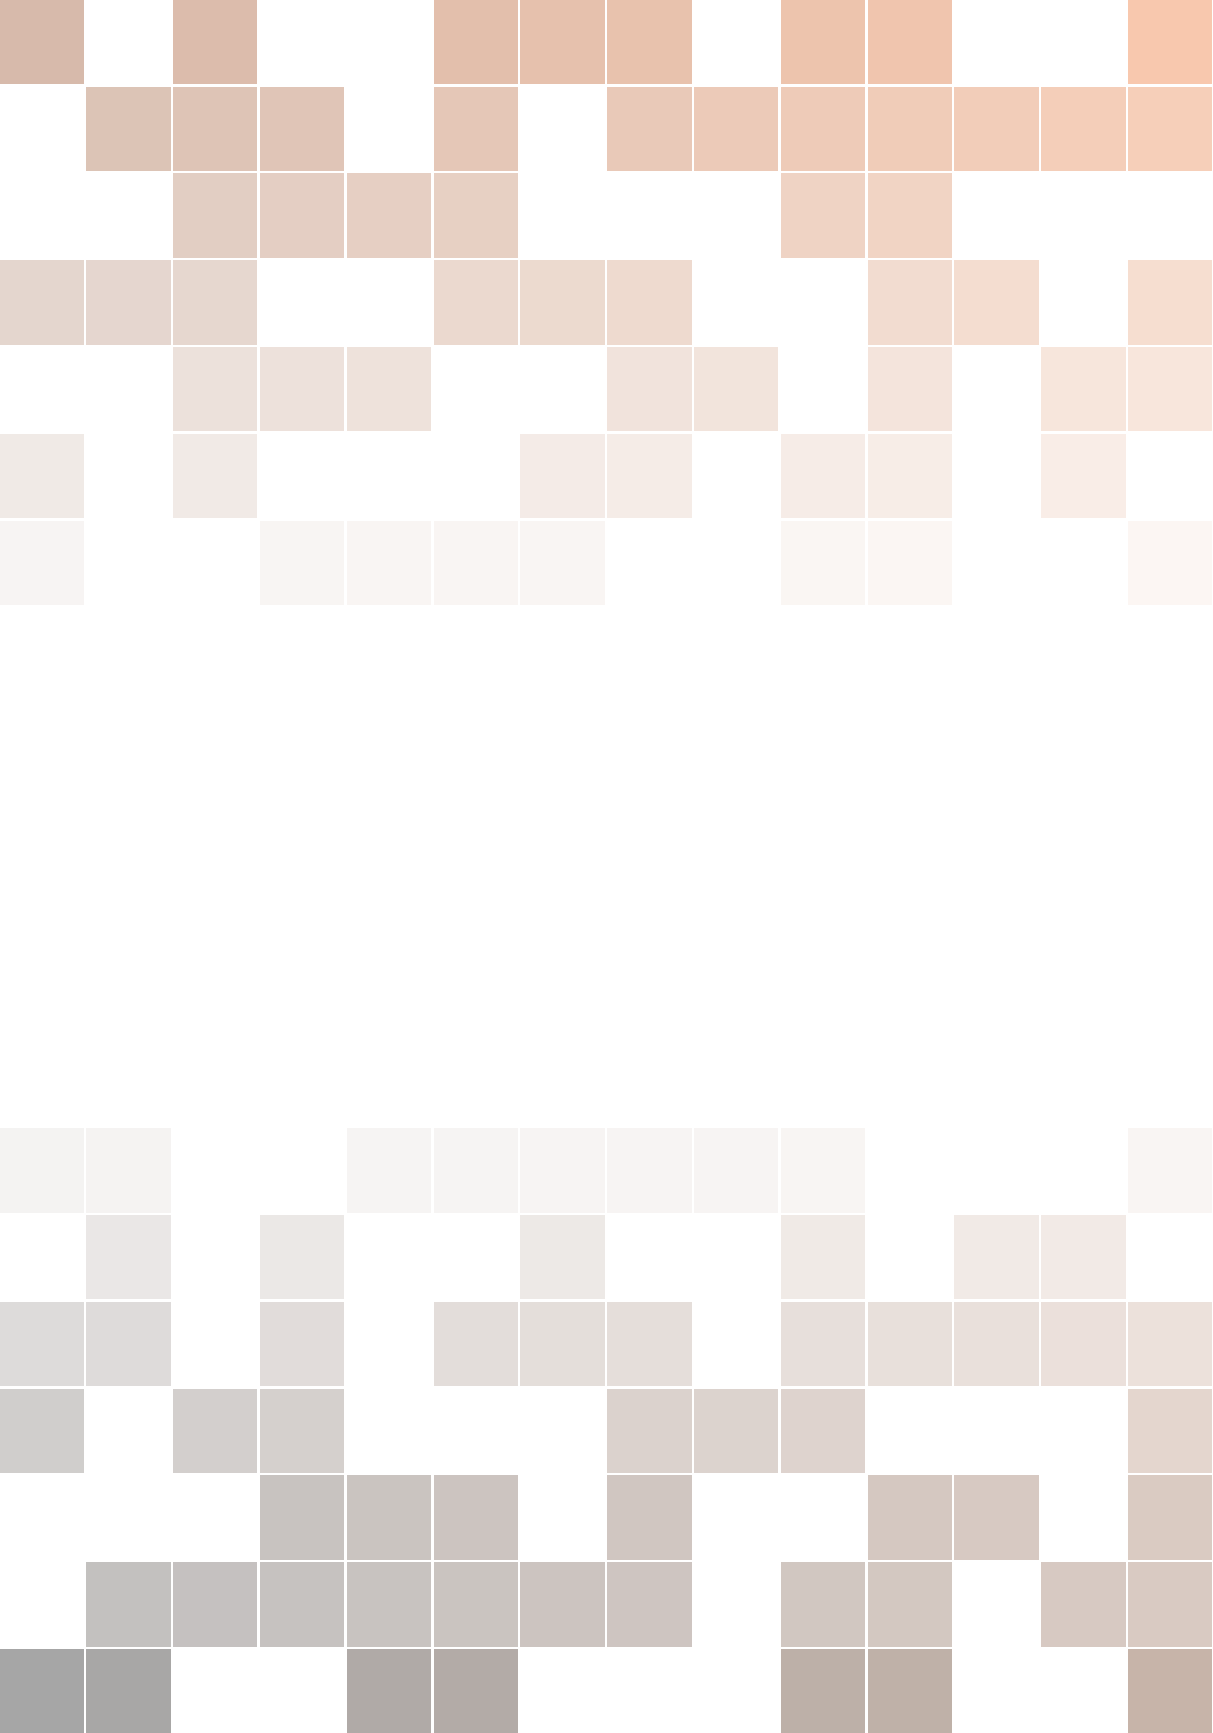
\includegraphics[width=\paperwidth]{images/background}}; % Background image
%\textsl{}
%      \draw[anchor=north] (midpoint) node [fill=ocre!30!white,fill opacity=0.6,text opacity=1,inner sep=1cm]{\Huge\centering\bfseries\sffamily\parbox[c][][t]{\paperwidth}{\centering Coding Interview Essentials\\[15pt] % Book title
%      {\Large - }\\[20pt] % Subtitle
%      {\huge Davide Spataro}}}; % Author name
%    \end{tikzpicture}};
%\end{tikzpicture}
%\vfill
%\endgroup


\includepdf[pages={2},fitpaper=true]{images/book_covers1.pdf}


	\usechapterimagefalse % If you don't want to include a chapter image, use this to toggle images off - it can be enabled later with \usechapterimagetrue

	%\chapterimage{images/header} % Table of contents heading image
	
	\pagestyle{empty} % No headers
	
	\tableofcontents % Print the table of contents itself
	
	\lstlistoflistings
	%\listoffigures
	%\listoftables

	%\cleardoublepage % Forces the first chapter to start on an odd page so it's on the right
	
	%pagestyle{fancy} % Print headers again
	
	%!TEX root = ../main.tex
%%%%%%%%%%%%%%%%%%%%%%%%%%%%%%%%%%
% Links: https://medium.com/@hazemu/finding-the-median-of-2-sorted-arrays-in-logarithmic-time-1d3f2ecbeb46
%
% Difficulty: Companies: 
%%%%%%%%%%%%%%%%%%%%%%%%%%%%%%%%%%

\chapter{Median of two sorted arrays}
\label{ch:median_sorted_arrays}
\section*{Introduction}

The median is one of the most basic and important concept in statistics and probability theory and
it finds applications in almost every field of science. It is defined as the value that split a
certain data set into two equally sized halves: the higher and the lower half. For example the median of the
dataset $\{1,3,4,6,10,12,19\}$ is $6$ because we have $3$ elements greater and $3$ elements smaller
than $6$. When the size of the dataset is even, such element does not exists and thus the median is defined as the mean of the two middle elements;
For instance given the dataset $\{1,3,4,6,8,10,12,19\}$, the median is $\frac{6+8}{2}=7$.  

The problem covered in this chapter is about finding the median from a dataset provided as two
separate input list of values (you can imagine, for instance, that each of the input set comes from
a separate thread as part of a multithreaded application to analyze a large dataset).
Despite an obvious solution exists that pretty follows from the definition of
median, this problem is considered to be hard to solve optimally in a coding interview context
as it requires non-trivial insights and careful implementation.
But, despite its daunting reputation has been asked often during coding interviews.

For the rest of the chapter we will go throught the problem statement, and then we dive deeper into the
problem by discussing a number of possible approaches that will make us go from a naive and
inefficient to a more sophisticated but optimal solution. 

\section{Problem statement}
\begin{exercise}
You are given two \textbf{sorted} arrays $A$ and $B$ of size $m$ and $n$, respectively. Your task is
to write a function that takes as input $A$ and $B$ and returns the median of the two sorted arrays.
$A$ and $B$ con be considered to be proper subsets of a third dataset $C = A \cup B$. 

	\begin{example}
		\hfill \\
		Given two sorted arrays:
		\begin{itemize}
			\item $A=[1,4,6,10,15]$
			\item $B=[2,3,5,6]$
		\end{itemize}
		The median is $5$ (see Figure \ref{fig:median_sorted_arrays:example2}).
	\end{example}

	\begin{example}
		\hfill \\
		Given two sorted arrays:
		\begin{itemize}
			\item $A=[1,4,6,10]$
			\item $B=[2,3,5,6]$
		\end{itemize}
		The median is $\frac{5+4}{2} = 4.5$ (see Figure \ref{fig:median_sorted_arrays:example1}).
	\end{example}

\end{exercise}

\begin{figure}
	\label{fig:median_sorted_arrays:example2}
	\centering
	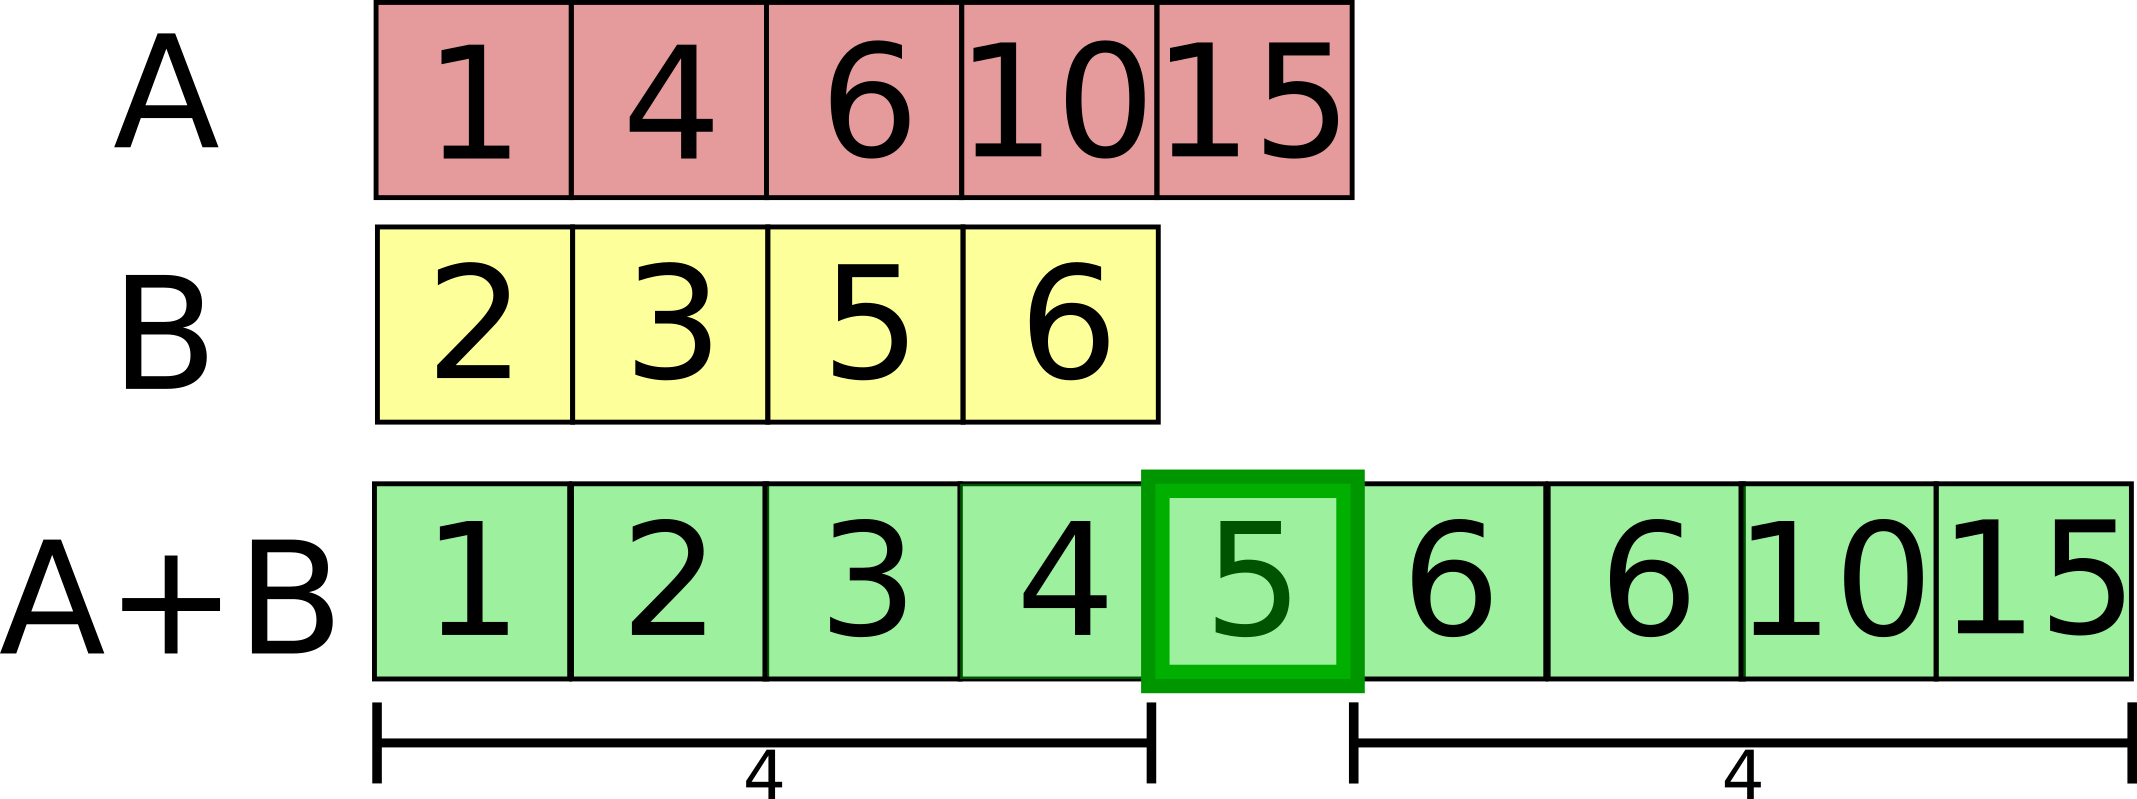
\includegraphics[scale=1.0]{sources/median_sorted_arrays/images/example2}
	\caption[Example of median of two sorted array.]{Example of median of two sorted array where the total number of elements is odd.}
\end{figure}

\begin{figure}
	\label{fig:median_sorted_arrays:example1}
	\centering
	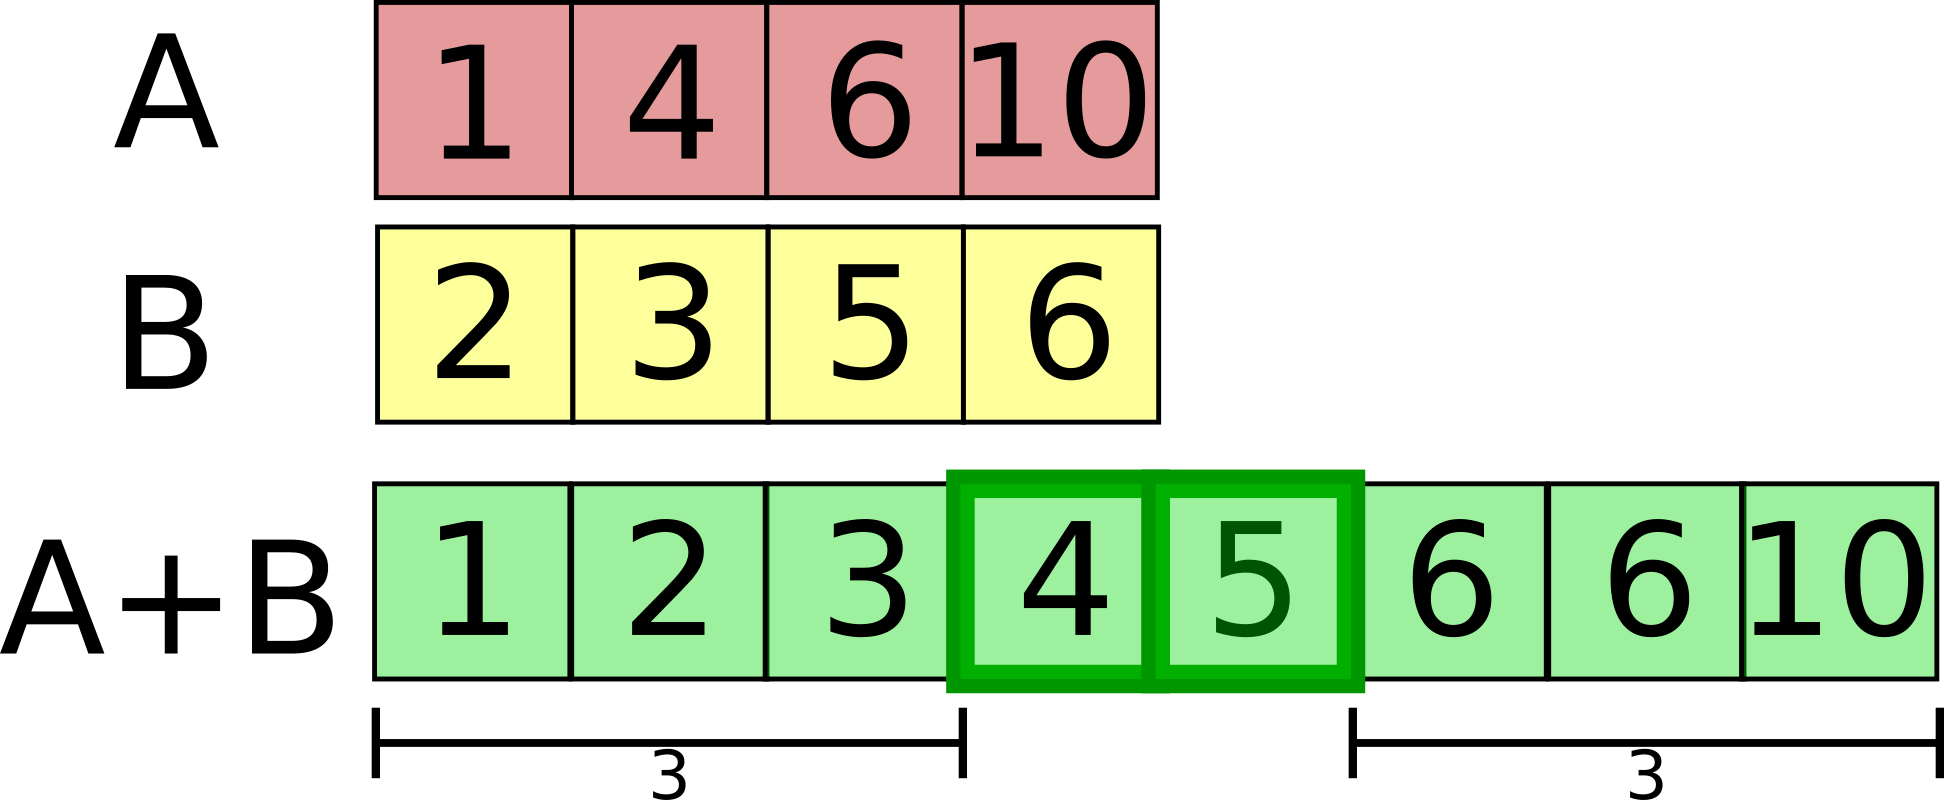
\includegraphics[scale=1.0]{sources/median_sorted_arrays/images/example1}
	\caption[Example of median of two sorted array.]{Example of median of two sorted array where the total number of element is even.}
\end{figure}


\section{Clarification Questions}

\begin{QandA}
	\item \begin{questionitem} \begin{question} Can $A$ or $B$ be empty?  \end{question} 	 
    \begin{answered}
		\textit{Yes, but you can assume that $|A \cup B| > 0$ i.e. at most one of the input array can be empty.}
	\end{answered} \end{questionitem}
	
\end{QandA}

\section{Discussion}
\label{median_sorted_arrays:sec:discussion}
Let's start our discussion by reviewing the concept of median. The median of a collection $C$ of $n$
elements is ($C_i$ represents the $i^{th}$ element of $C$):
\begin{itemize}
	\item $C_{\frac{n}{2}}$ if $n$ is odd (see Figure \ref{fig:median_sorted_arrays:example1})
	\item $\frac{C_{ \lfloor \frac{n}{2} \rfloor    }+C_{ \lceil \frac{n}{2} \rceil   }}{2}$ if $n$ is even (see Figure
	\ref{fig:median_sorted_arrays:example2})
\end{itemize}
In simpler terms the median of a sorted collection is the element which divides the collections into
two equally sized halves, left and right, each with the same number of elements. 
If $n$ is even, clearly such element does not exists and thus the median is the defined to be the mean of the two middle
elements as shown in Figure \ref{fig:median_sorted_arrays:example1}.
Additionally, notice that because the collection is sorted then all the elements in the left half are smaller or equal then
the median and all the elements on the right half are larger. 

\subsection{Brute-force}
\label{median_sorted_arrays:sec:bruteforce}
Armed with the definition of median, we can immediately devise a simple and effective approach to
find it given the two input sorted arrays. The only difference between the problem statement and the
definition of median is that we are given two sorted arrays and not just one. Therefore it is
natural that the very first thing that should come to mind is to:
\begin{enumerate}
	\item create a third array $C = A \cup B$, which is the concatenation of the two input arrays
	\item proceed by sorting $C$,
	\item calculate the median (and not forgetting to take into consideration the parity of $|C|$)
\end{enumerate}

This approach is clearly correct as it is basically a direct consequence and application of the
definition of median given above, but it is far from being optimal, as we will see below. Listing
\ref{list:median_sorted_naive} shows a C++ implementation of this idea. Time and space complexities
of this approach are $O((n+m)log(n+m))$(because of sorting) and $O(s+m)$(space required by the third
array), respectively. Despite being suboptimal this solution has the benefit of being very short (only a few lines)
and easy to read, explain and understand.

\lstinputlisting[language=c++, caption={Naive implementation of solution to the problem of finding the median of two sorted arrays.},label=list:median_sorted_naive]{sources/median_sorted_arrays/median_sorted_arrays_solution1.cpp}


\subsection{Brute-force improved}
\label{median_sorted_arrays:sec:bruteforce_improved}
The brute-force approach can be improved a bit if we use the fact that the arrays are already
sorted. In the approach described in Section \ref{median_sorted_arrays:sec:bruteforce} we do not use
this fact and therefore we are forced to sort the entire array $C$ that we created by blindly juxtaposing $A$ and $B$ one after the other.
By taking advantage of the fact that the inputs are sorted we can create the array $C$ in a smarter way,
so that it is already sorted. In order to do so we will use the fact that you can merge two sorted array into a third sorted array in linear time.
You might be already familiar with this idea if you know how the famous merge-sort algorithm\cite{wiki:mergesort} works as the same operation is one of its two basic building blocks.
Listing \ref{list:median_sorted_naive_2} shows how this idea can be coded in C++. Notice how most of the code is now taken by the \inline{std::vector<T> mergeSortedArrays(const std::vector<T> &A,
const std::vector<T> &B)} function that 
is responsible for taking two sorted arrays (pay attention to the \inline{assert}) as input and returning a third sorted one. 

\lstinputlisting[language=c++, caption={Naive implementation of solution to the problem of finding the median of two sorted arrays using the merge part of merge-sort algorithm.},label=list:median_sorted_naive_2]{sources/median_sorted_arrays/median_sorted_arrays_solution2.cpp}

The time and complexities of this version are both $O(n+m)$, much better than the one from the solution presented in
Section \ref{median_sorted_arrays:sec:bruteforce} but, it is still suboptimal as this problem can be
solved in logarithmic time. We are going to see how in Section \ref{median_sorted_arrays:sec:log}.

\subsubsection{Merge sorted arrays in linear time}
How exactly can we merge two sorted arrays $X$ and $Y$ into a third sorted array $Z$ in linear time? 
The idea behind is that we can build $Z$ incrementally starting from an empty array, and at each step of the process
inserting one of the elements of $X$ or $Y$ depening on which one of the two containts the smallest element at that moment.
In the implementation of \inline{mergeSortedArrays} this is achieved by using two iterators, \inline{itX} and \inline{itY} 
each pointing to the next element of $X$ and $Y$ to be inserted in $Z$, respectively.
The \inline{while} loop is responsible for comparing the two elements pointed by the iterators and always inserting the smallest one
into $Z$.  Once an element is merged in the final array, the corrensponding iterator is incremented so the next value will be considered at the next iteration.
When one of the two iterators its the end of its array, then all we are left are the remaining elements of the other collection that we can at this point blindly insert into $Z$ because they are sorted 
(see the last two \inline{while} loops in the code).
Figure \ref{fig:median_sorted_array:mergearray} shows all the steps that are necessary to perform the merging for the arrays:
$X = \{1,3,5,8,15\}$ and $X = \{2,4,7\}$. At step $1$ (Figure \ref{fig:median_sorted_array:mergearray0}) $Z$ is initially empty and \inline{itA} and \inline{itB} point to the beginning of $X$ and $Y$, respectively.
Because the element pointed by itA is smaller, it is selected for merging and thus itA is incremented.
At step $2$ (Figure \ref{fig:median_sorted_array:mergearray1}) the element pointed by itB is smaller, and as in the previous step, it is merged in $Z$ and itB is incremeneted.
The same operations are performed for all the steps depicted in Figures 
\ref{fig:median_sorted_array:mergearray2},
\ref{fig:median_sorted_array:mergearray3},
\ref{fig:median_sorted_array:mergearray4},
\ref{fig:median_sorted_array:mergearray5} and \ref{fig:median_sorted_array:mergearray6}.
Eventually itB goes out of range signalling that all the element in $Y$ have been processed (see Figure \ref{fig:median_sorted_array:mergearray6}).
At this point then, as shown in Figure \ref{fig:median_sorted_array:mergearray7} we can safely merge all the element in $X$ into $Z$ that is now ready to be returned (see Figure \ref{fig:median_sorted_array:mergearray8}).

\begin{figure}
	\centering
	\begin{subfigure}[b]{0.45\textwidth}
		\centering
		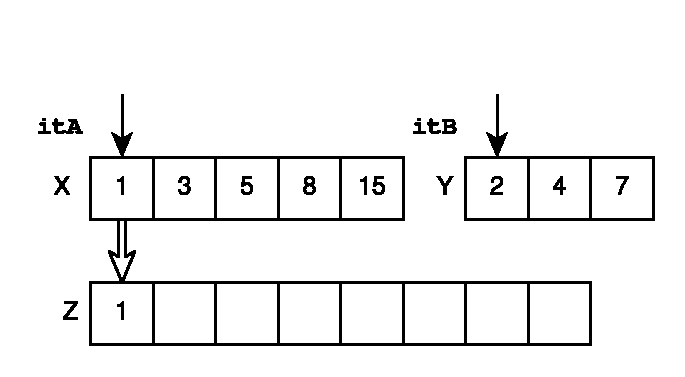
\includegraphics[trim=0 0 0 45,clip,width=\textwidth]{sources/median_sorted_arrays/images/mergearrays0}
		\caption{Step $1$: $Z$ is initially empty. itX and itY points to the beginning of $X$ and $Y$, respectively. The element pointed by itX is merged as it is smaller. itX is advanced by one position.}
		\label{fig:median_sorted_array:mergearray0}
	\end{subfigure}
	\hfill
	\begin{subfigure}[b]{0.45\textwidth}
		\centering
		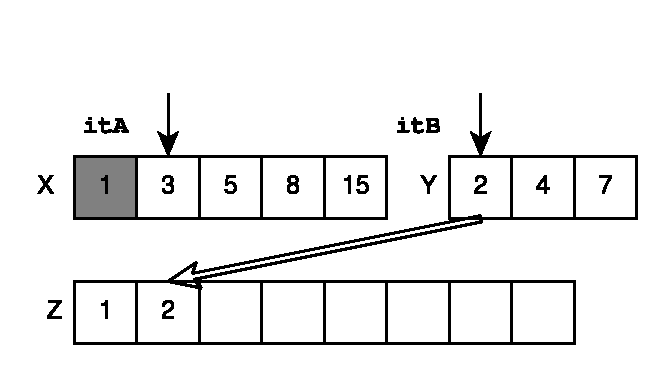
\includegraphics[trim=0 0 0 45,clip,width=\textwidth]{sources/median_sorted_arrays/images/mergearrays1}
		\caption{Step $2$: itY is smaller than itX, thus it is the one being merged. itB is also advanced by one position. }
		\label{fig:median_sorted_array:mergearray1}
	\end{subfigure}
	\hfill

	\begin{subfigure}[b]{0.45\textwidth}
		\centering
		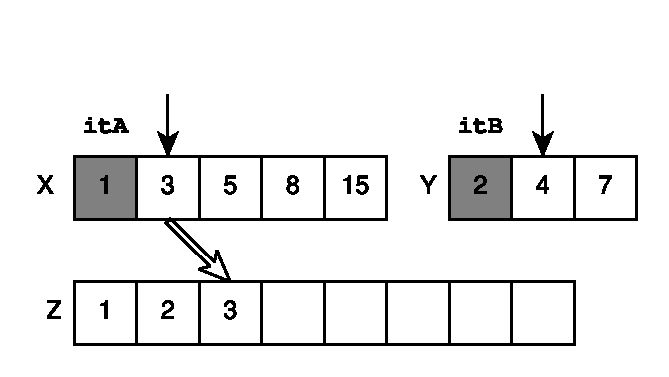
\includegraphics[trim=0 0 0 45,clip,width=\textwidth]{sources/median_sorted_arrays/images/mergearrays2}
		\caption{Step $3$: itX is smaller than itY, thus it is the one being merged. itX is also advanced by one position.}
		\label{fig:median_sorted_array:mergearray2}
	\end{subfigure}
	\hfill
	\begin{subfigure}[b]{0.45\textwidth}
		\centering
		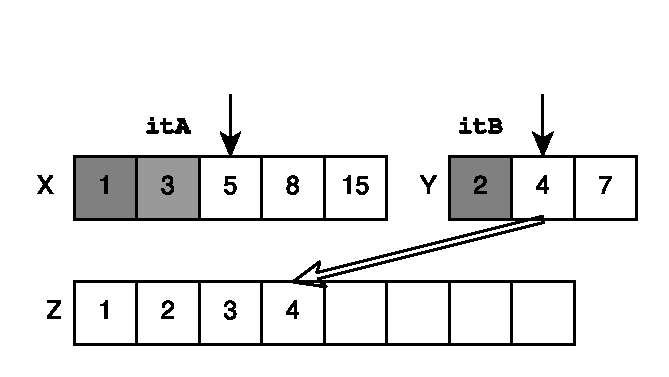
\includegraphics[trim=0 0 0 45,clip,width=\textwidth]{sources/median_sorted_arrays/images/mergearrays3}
		\caption{Step $4$: itY is smaller than itX, thus it is the one being merged. itB is also advanced by one position. }
		\label{fig:median_sorted_array:mergearray3}
	\end{subfigure}
	\hfill

	\begin{subfigure}[b]{0.45\textwidth}
		\centering
		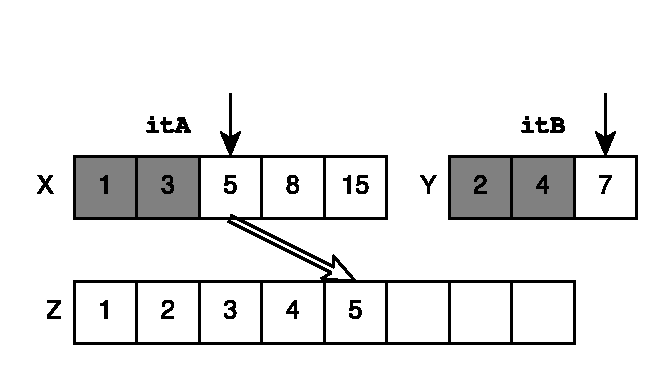
\includegraphics[trim=0 0 0 45,clip,width=\textwidth]{sources/median_sorted_arrays/images/mergearrays4}
		\caption{Step $5$:  itX is smaller than itY, thus it is the one being merged. itX is also advanced by one position.}
		\label{fig:median_sorted_array:mergearray4}
	\end{subfigure}
	\hfill
	\begin{subfigure}[b]{0.45\textwidth}
		\centering
		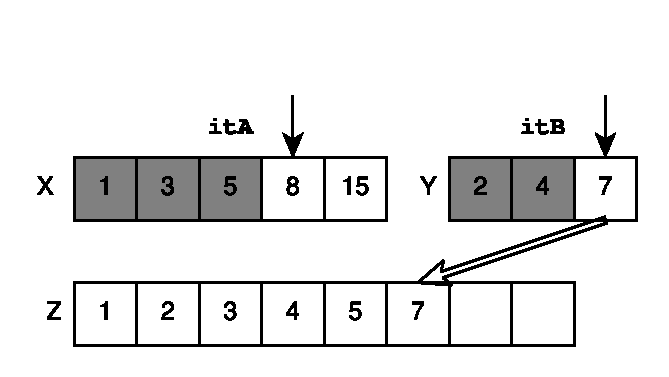
\includegraphics[trim=0 0 0 45,clip,width=\textwidth]{sources/median_sorted_arrays/images/mergearrays5}
		\caption{Step $6$:itY is smaller than itX, thus it is the one being merged. itB is also advanced by one position.}
		\label{fig:median_sorted_array:mergearray5}
	\end{subfigure}
	\hfill

	\begin{subfigure}[b]{0.45\textwidth}
		\centering
		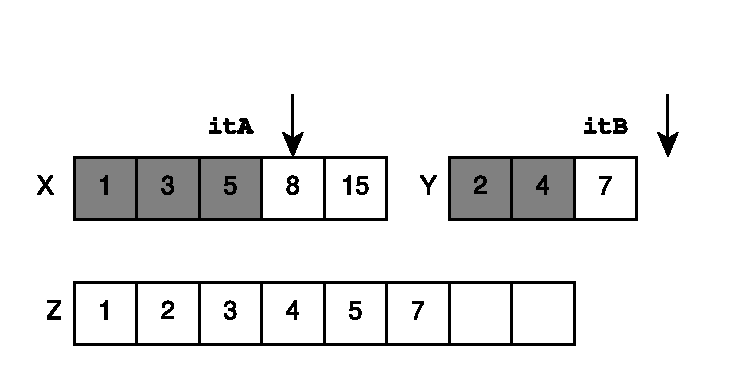
\includegraphics[trim=0 0 0 45,clip,width=\textwidth]{sources/median_sorted_arrays/images/mergearrays6}
		\caption{ itY now  points to the past-the-end element of $Y$. There are no more element of $Y$ to merge.}
		\label{fig:median_sorted_array:mergearray6}
	\end{subfigure}
	\hfill
	\begin{subfigure}[b]{0.45\textwidth}
		\centering
		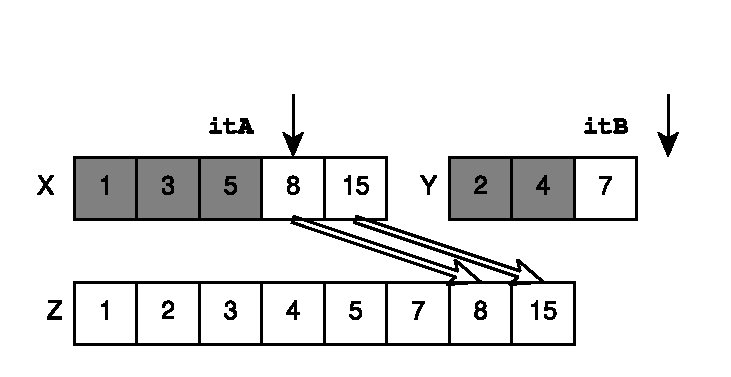
\includegraphics[trim=0 0 0 45,clip,width=\textwidth]{sources/median_sorted_arrays/images/mergearrays7}
		\caption{Step $7$: All the remaning element from the current location of itX to the end of X are merged into $Z$. }
		\label{fig:median_sorted_array:mergearray7}
	\end{subfigure}
	\hfill
	\begin{subfigure}[b]{0.45\textwidth}
		\centering
		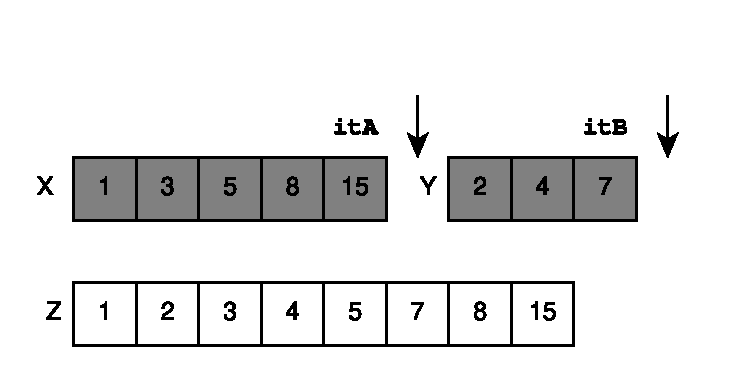
\includegraphics[trim=0 0 0 45,clip,width=\textwidth]{sources/median_sorted_arrays/images/mergearrays8}
		\caption{All the elements of $X$ and $Y$ have been merged. $Z$ contains the element of $X \cup Y$ and it is sorted.}
		\label{fig:median_sorted_array:mergearray8}
	\end{subfigure}
	\caption[Example of merging two sorted arrays.]{This figure shows how two sorted arrays can be merged into a third sorted array in linear time. The hollow indicates which element at that step is selected to go into the third array. Notice that the iterator associated with that element is then moved forward. Already merged cells are }
	\label{fig:median_sorted_array:mergearray}
\end{figure}


\subsection{Logarithmic solution}
\label{median_sorted_arrays:sec:log}
If we want to improve the $O(n+m)$ solution we have at hand at this point we need to abandon the idea of constructing a third array containing all the elements from the inputs.
There is no way this can be done in less than linear time as one must at least access the input element once.
Turns out, we do not actually need to have the array $C$ at all. 

The key insights are:
\begin{itemize}
	\item we know exactly what the size of the merged array $C$ would be: $n+m$.
	\item we also know that the part of $C$ to the left of the median, $C_l$ would be made up from elements among the smallest values of $A$
	and $B$. These values also lie in the left portions of $A$ and $B$. For instance, w.r.t. the example in Figure \ref{fig:median_sorted_arrays:example2} we
	can see that the left half (the first $5$ elements) of $A \cup B$ is made from the first two elements
	of $A$ and the smallest $3$ elements of $B$. Because $C$ will be sorted, only the smallest
	elements of $A$ and $B$ will can be part of $C_l$.
\end{itemize}
The problem is that we do not know exactly how many elements of $A$ will be part $C_l$ but if we do, then, we also know immediately how many elements of $B$ go to $C_l$
and at that point we can calculate the median.
We cannot find directly how many elements  of $A$ contributes to $C_l$, but we can test farily easily if the first $i$ elements do.
Let's suppose we try to make $C_l$ by using $i$ elements from the left portion of $A$.
Because $|C|=n+m$ then $|C_l| = \frac{n+m}{2} = i+j$ where $j$ is the number of elements from the left part of $B$ contributing to $C_l$. 
Thus if we take $i$ elements from $A$ we need to take $j = (n+m)-i$ elements from $B$. 
Once $i$ and $j$ are decided, we also know that the last element of $C_l$, will be the maximum element among the first $i$ elements of $A$ and the first $j$ elements of $B$.
From these arguments follows that the right half of $C$, $C_r$,  contains all the remaining $n-i$ elements of $A$ and $m-j$ of $B$, 
and also that the first element of $C_r$ will be the smallest element among them.
Given:
\begin{itemize}
	\item $M_l$ is the largest elements among the $A[i]$  $B[j]$
	\item $m_r$ is the smallest element among the $A[i+1]$  $B[j+1]$
\end{itemize} 
then if $i$ is indeed the right amount of element from $A$ belonging to $C_l$ then, $M_l \leq m_r$.
If $M_l > m_r$ then we need to understand whether we took too many or too few elements from $A$ to be part of $C_l$. 
We can check this by checking whether  $M_l$ belongs to $B$ or $A$, respectively. 
Thus if $A[i] > B[j]$ we reduce or increase $i$ by doing $r = r-1$. 
Conversely if $A[i] < B[i]$ then $i$ is increased by moving the left boundary of the binary search range: $l = l+1$.

Listing \ref{list:median_sorted_binary} shows an implementation of the idea above.
\lstinputlisting[language=c++, caption={Binary search solution to the \textit{median of two sorted arrays} problem.},label=list:median_sorted_binary]{sources/median_sorted_arrays/median_sorted_arrays_solution3.cpp}



https://leetcode.com/problems/median-of-two-sorted-arrays/ complete this code first
use binary search to find i
l , r is the range of elements of A initially l = 0 r = min(n, (n+m)/2)
i = l+r/2
j = n+m-i
if max among A[i] and B[j] <= min A[i+1],B[j+1] we have a median
otherwise 
if A[i] > B[j] then r = i-1
else l = i+1

	
	%%%%%%%%%%%%%%%%%%%%%%%%%%%%%%%%%%%%%%%%%%%%
	%               Appendices
	%%%%%%%%%%%%%%%%%%%%%%%%%%%%%%%%%%%%%%%%%%%%
	
	\chapter{Appendices}
	% @Author: Davide Spataro
% @Date:   2020-10-25 
% @Last Modified by:   Davide Spataro
% https://www.topcoder.com/community/competitive-programming/tutorials/dynamic-programming-from-novice-to-advanced/
% file:///home/knotman/Downloads/DYNAMIC_PROGRAMMING_-_ITS_PRINCIPLES_APPLICATIONS_.pdf
% http://smo.sogang.ac.kr/doc/bellman.pdf 
\section*{Dynamic Programming}
\label{sect:appendix:DP}

Dynamic programming (DP) is a popular technique for solving a certain class of
optimization problems efficiently and is accredited to the American Scientist
Richard Bellman\cite{bellman1954}. He conied the term DP in the context of
solving problems involving a serie of best decision one after the other. 
The word \textit{programming} can be a bit deceiving for
computer scientist of programmers in general but it has really little to do with
computer programming and it is infact intended as a set of rules to 
follow to solve a certain problem and it is refeered specifically to the
solution to find an optimal military schedule for logistics (and has more or
less the same meaning as linear programming or linear optimization).  These rules can of course be coded and
executed by a computer but can be easily followed on paper for instance. 
Dynamic programming is better thought as an optimization approach rather than an
method or framework where a complex optimization problem is transformed into a sequence of
smaller (and simpler) problems. The very essence of DP is its multi-stage
optimization procedure. DP does not provide directly with the
instruction on how to solve a particular problem, but instead provides a general
framework that requires creativity and non trivial effort/insights so that a
problem formulation can be adapted and casted within the DP framework bounds.
This is possibly the reason why DP is considered a rather hard topic and it is
particularly feared during interviews. 

This chapter is not intended to be a full treatement of DP, and we will
introduce and describe it to the level that is necessary to understand and
better tackle DP interview problems. For a more comprenshive material on DP
please refer to \cite{bellman1954, cormen2009}.

The gist of the DP approach is that we aim at breaking down a problem into
simpler sub-problems recursively. If it is possible to do so, then the problem
at hand is said to have the \textbf{optimal substructure} property i.e. it can
be solved by using optimal solution to subproblems. But having the optimal
substructure property alone is not enough to prefer a DP approach to another
when trying to solve the same problem. This is because DP really shines when a
problem also exposes the \textbf{overlapping subproblems} property i.e. when the
subproblems are reused several times. A classic example if the
Fibonacci Sequence. In order to calculate $F(n)$ we need to solve two subproblems:
$F(n-1)$ and $F(n-2)$ and adding them up. But for solving $F(n-1)$ we need to
solve $F(n-2)$ \textbf{again}. The value for the subproblem $F(n-2)$ is thus
reused and this makes the Fibonacci problem exposed the optimal substructure
property. 
Dynamic programming takes care of this fact by making sure of solving each
subproblem only once. Usually this can be achieved into two ways:
\begin{description}
    \item [Top-down] This is usually the easiest of the two, by being a direct
    derivation from the recursive formulation of the problem. If the problem can
    be formulated recursively in terms of solution then solution to subproblems
    can be \textit{memoized}\footnote{From the latin word \textit{memorandum}
    which means to be remembered. It is basically a way of remembering the
    result of a function for a certain set of inputs call by storing it in a
    cache.} in a cache. 
    When a subproblem is reused then the
    (potentially expensive) recursive call is avoided and the cached result is
    returned instead. 
    \item [Bottom-up] We can try to reformulate the problem by twisting and
    massaging  the  recursive formulation so that the subproblems are solved
    first (thus effectively removing the recursion) and build the solution to
    the bigger problem from the bottom. This is usually done by working in a
    sort of tabular form where entries of the table for larger problems are
    filled by using  entries for solution to smaller problems that we have
    already solved. For instance, when solving the problem of finding the
    $10^{th}$ Fibonacci number $F(10)$, we can start from the known values for
    $F(0)$ and $F(1)$ and working our way up to $F(2)$  by using $F(1)$ and
    $F(2)$. Once F(2) is ready we can move up to F(3), and so on when we have
    the values for $F(8)$ and $F(9)$ we proceed with calculating $F(10)$.
\end{description}

DP has found application in many field of science such as Control theory,
Bioinformatics AI and operations research. There are a number of problems in
computer science that can be solved by using DP such as the 
\begin{itemize}
    \item Longest Common (or increasing) Subsequence
    \item Weighted Interval Scheduling
    \item Chain Matrix Multiplication
    \item Subset sub
    \item String edit distance
    \item Coin change
    \item 0/1 knapsack problem
    \item Graph shortest path
\end{itemize}

In the next section we will shortly review a number of DP problem focusing on
the key ideas that allow a problem to be approached and solved  using DP.

\subsection*{Fibonacci Sequence}
Computing the $n^{th}$ number of the Fibonacci sequence is probably one of the
most common introductionary example of DP. The Fibonacci sequence recursive
formulation is ready to be solved using a top-down DP approach. Listing
\ref{list:app:dp:canonical} shows a C++ function that calculated the $n^{th}$ Fibonacci
number.
\lstinputlisting[language=c++, caption={Canonical recursive C++ implementation of a function returning the $n^{th}$ Fibonacci number.},label=list:app:dp:canonical]{/home/dspataro/git/algorithm_articles/sources/appendices/fibonacci_canonical.cpp}
Notice that for instance when $F(6)$ a call tree is produced where the same call
is repeated more than once as shown in the list below. $F(2)$ has been
calculated $5$ times!
\begin{itemize}
    \item $F(6) = F(5)+F(4)$
    \item $F(6) = (F(4)+F(3)) + (F(3)+F(2))$
    \item $F(6) = ((F(3)+F(2))+(F(2)+F(1))) + ((F(2)+F(1))+(F(1)+F(0)))$
    \item $F(6) = (((F(2)+F(1))+(F(1)+F(0)))+((F(1)+F(0))+F(1))) + (((F(1)+F(0))+F(1))+(F(1)+F(0)))$
    \item $F(6) = ((((F(1)+F(0))+F(1))+(F(1)+F(0)))+((F(1)+F(0))+F(1))) + (((F(1)+F(0))+F(1))+(F(1)+F(0)))$
\end{itemize}

Listing \ref{list:app:dp:fib} can be improved dramatically if we memoize the function calls
that have been already calculated. This way no duplicate work is done. W.r.t the
previous example, from the second time the value of $F(2)$ is needed, no
additional work is done, as the value in the cache is returned.
\lstinputlisting[language=c++, caption={Canonical recursive top-down Dynamic Programming C++ implementation of a function returning the $n^{th}$ Fibonacci number.},label=list:app:dp:fib]{/home/dspataro/git/algorithm_articles/sources/appendices/fibonacci_dp_top_down.cpp}

	%\section{Prefix sum}
\label{sect:appendix:prefix_sum}
In computer science, the prefix sum, cumulative sum, inclusive scan, or simply scan of a sequence of numbers x0, x1, x2, ... is a second sequence of numbers y0, y1, y2, ..., the sums of prefixes (running totals) of the input sequence:
	%% @Author: Davide Spataro
% @Date:   2020-03-30 17:18:14
% @Last Modified by:   Davide Spataro
% @Last Modified time: 2020-03-30 17:28:08
\section{Binary Search}
\label{sect:appendix:binary_search}
\lipsum{1}
    %%%%%%%%%%%%%%%%%%%%%%%%%%%%%%%%%%%%%%%%%%%%
	%               BIBLIOGRAPHY
	%%%%%%%%%%%%%%%%%%%%%%%%%%%%%%%%%%%%%%%%%%%%
	
	%\chapter*{Bibliography}
	\addcontentsline{toc}{chapter}{\textcolor{ocre}{Bibliography}}
	\printbibliography	
	
%%%%%%%%%%%%%%%%%%%%%%%%%%%%%%%%%%%%%%%%%%%%
%               INDEX
%%%%%%%%%%%%%%%%%%%%%%%%%%%%%%%%%%%%%%%%%%%%	
	\cleardoublepage
	\phantomsection
	\setlength{\columnsep}{0.75cm}
	\addcontentsline{toc}{chapter}{\textcolor{ocre}{Index}}
	\printindex


	%\backmatter

\end{document}
